% Chapter 2

\chapter[Literature Review]{Literature Review} % Main chapter title

\label{Chapter2} % For referencing the chapter elsewhere, use \ref{Chapter1} 

%----------------------------------------------------------------------------------------

\section{Overview}
This section presents a review of some of the literature from the field of swarm robotics, beginning with some general summaries of the field's fundamentals, followed by a number of specific pieces of research from topic areas with particular relevance to this project. These areas include human-swarm interaction, robotics debugging, and robotics-focused augmented reality research. Finally a number of papers which connect augmented reality techniques directly to swarm robotics, and are therefore well aligned with the aims of this project, are discussed and critiqued. The results of this literature survey informed the project direction significantly, and formed the basis for many of the design and implementation decisions made later on. This literature review is also presented with the aim of providing the reader with the base of knowledge required to better understand the project.

%----------------------------------------------------------------------------------------

\section{Swarm Intelligence and Swarm Robotics} \label{GeneralSwarmRobotics}
An understanding of the fundamental concepts of Swarm Robotics, and to a lesser extent Swarm Intelligence, was deemed key to producing an application that is useful in practice, and will help a reader to better understand the purpose and aims of the project. A deep understanding of the technical details of specific swarm behaviours or implementations is not a priority for understanding this project, as the application aims to be more broadly applicable to a wide range of swarm systems. Emphasis has instead been placed on understanding the general classification of swarm robotic systems, relevant problem domains, and recurring concepts, so that the system might better serve researchers in the field.

Sahin \cite{Sahin:2004} presents a summary of the key concepts of swarm robotics, and attempts to offer a coherent description of the topic. He notes that a key difference from other multi-robot systems is the lack of centralised control, and the idea that desired swarm level behaviour should emerge from simple local interactions between robots, and between the robots and their environment. He also notes some of the key motivators behind Swarm Robotics research, stating that a swarm robotics system would ideally exhibit ``\textit{robustness}'', ``\textit{flexibility}'' and ``\textit{scalability}'' \cite{Sahin:2004}. Robustness refers to the swarm's ability to continue to function should one or more individual swarm members suffer a failure of some kind. Flexibility refers to the swarm's ability to adapt to changes in the environment without the need for re-programming. Scalability describes the idea that a swarm should be functional at a range of sizes, and that ideally the number of robots in the swarm could be increased or decreased depending on the demands of the task. These descriptors should be taken into account by the design of the system presented in this project. In order for the system to be able to work well with robust, scalable swarms it should adapt easily to variation in the number of robots being monitored. Newly detected robots should therefore be incorporated seamlessly. The video feed component of the system will allow a user to see the environment the swarm is interacting with and observe how robots respond to changes within it, and therefore judge the extent to which the swarm exhibits flexibility.

Sahin \cite{Sahin:2004} goes on to describe several classes of application for which Swarm Robotics systems might be well suited. Tasks that cover a region could benefit from a swarm's ability to distribute physically in a space according to need. Dangerous tasks could benefit from the relative dispensability of individual robots in the swarm; should one be damaged or destroyed the swarm could continue to function, and it would be less costly than the loss of a single, complex, expensive robot. Tasks requiring scalability are good candidates, as discussed before, and tasks that require redundancy are also highlighted, as swarm systems should have the ability to degrade gracefully, rather than suffering a single catastrophic failure. Through this generalisation of the application areas, insight can be gained into the kinds of work swarm robotics researchers are likely to be doing, and this should inform the design of the application. Overall Sahin's paper \cite{Sahin:2004} provides a coherent, succinct overview of the field, and although it is now over a decade old the concepts covered remain relevant.

The book `\textit{Swarm Intelligence: From Natural to Artificial Systems}', by Bonabeau, Dorigo and Theraulaz \cite{Bonabeau:1999}, provides in its introductory chapter a good overview of the biological concepts and animal behaviours which inspired much of the research that led to the creation of the field of swarm intelligence. Fundamental concepts such as self-organisation and decentralised control are discussed. In order to be a useful tool in the swarm robotics research space, it is important that the system developed during this project does not violate these core principles of the swarm robotics paradigm. Therefore the system should not facilitate low level control of the robots or allow for forms of communication and data exchange that might invalidate the self-organising, decentralised nature of the swarm's behaviour. The later chapters \cite{Bonabeau:1999} provide a detailed look at several key insect behaviours, and how mathematical models and algorithms can be derived to mimic them. An understanding of these behaviours and models can offer insight into what information the application might need to expose to allow a user to validate the correct operation of a swarm behaviour based on these concepts. A number of these algorithms focus or rely on data related to the position and movement of individuals within the swarm, and the swarm as a whole. The system developed during this project should reflect the importance of positional data and provide features which aid the user in interpreting it.

In a more modern work, Brambilla et al. \cite{Brambilla:2013} focus heavily on the engineering practicalities of designing, implementing and testing swarm robotic systems. The authors then apply this focus as a means by which to classify and critique a large body of swarm robotics research, noting that although much work has been carried out regarding the design and analysis of swarm behaviours, other areas including maintenance and performance measurement are heavily lacking in research contributions \cite{Brambilla:2013}. Debugging can be considered a maintenance task, and the system developed in this project has potential in both maintenance and performance measurement applications. It is hoped therefore that this work might contribute to this area of the field, by investigating through implementation the practicalities of a generalised swarm maintenance and observation software application. The authors \cite{Brambilla:2013} later note that human-swarm interaction remains an open issue, and will be key to realising functional, real-world swarm robotic systems. They identify a number of works related to human-swarm interaction, almost all of which focus on the task of controlling a robot swarm, and investigate different methods by which a user might insert data into the swarm system. Little consideration appears to be given, both in this paper and throughout the literature, to the task of monitoring a swarm, and best practices for retrieving information in a manner that is useful to a human operator.

%----------------------------------------------------------------------------------------

\section{Human Swarm Interaction} \label{HumanSwarmInteraction}
This project focuses on a piece of software which forms an interface between a human operator and a robot swarm. A relevant area of research is therefore Human-Swarm Interaction (HSI). Research in this area focuses on the different ways in which humans and robot swarms can interact, the different roles humans take whilst interacting with robot swarms, and the best practices for facilitating this interaction given different aims, and different user roles (developer, researcher, end user, etc.). The two key challenges of HSI are \textit{control} and \textit{monitoring}. The former refers to how best to allow a human operator to direct the behaviour of a decentralised swarm, whilst the latter refers to how best to retrieve data from a swarm and present it in a useful, human readable manner. This project is related to debugging robot swarm behaviours, which is primarily a swarm monitoring task, and therefore this section focuses on the monitoring side of HSI.

In their paper `\textit{Human Interaction with Robot Swarms: A Survey}' \cite{Kolling:2016} Kolling at el. begin by noting the lack of research into methods for interfacing humans and robot swarms. They suggest that real-world applications for swarm robotics systems are now within reach, and that discovering effective methods for allowing humans to control and/or supervise swarms is a key barrier to realising these systems. The paper \cite{Kolling:2016} provides a detailed analysis of human swarm interaction from a number of different perspectives. Of relevance to this project is the statement on page 15 that ``\textit{Proper supervision of a semiautonomous swarm requires the human operator to be able to observe the state and motion of the swarm, as well as predict its future state to within some reasonable accuracy}'' \cite{Kolling:2016}. This statement lends credence to the aims of this project, as swarm supervision and swarm debugging are highly comparable tasks; both involve observing the swarm whilst performing its task and determining the validity of the behaviour observed. The system developed in this project should allow the state of the swarm, including the internal state of individual robots, to be observed simultaneously with the physical positions and motions of the robots within their environment. The paper \cite{Kolling:2016} goes on to suggest that by observing the swarm over time the human operator will be able to provide `\textit{appropriate control inputs}'. In the case of this application, rather than providing control input, the human operator will be seeking to identify faults, and provide appropriate corrections to the system, however the concept of state visualisation remains relevant.

Rule and Forlizzi \cite{Rule:2012} present a thorough examination of the complexities of human robot interaction (HRI) when dealing with multi-robot (and multi-user) systems. Much of the paper focusses on control methods, which are not directly applicable to this project, however section 2.4 titled \textit{Salience of Information} discusses the task of designing interfaces for displaying information about multi-robot systems to a human operator in a manner which is both information dense and rapidly understandable. The authors note that the use of colour has been shown to improve interface readability \cite{Christ:1984}, and that the brain has been shown to process text faster than images \cite{Carney:1998}, hence complex icons should be avoided. These ideas should be incorporated into the design of the application user interface for this project. A range of different designs could be explored, including finding a balance between the amount of information displayed graphically, and the amount displayed textually, and deciding whether to use colour to differentiate between individual robots, or to differentiate between different types of data, or a combination of both.

The authors \cite{Rule:2012} then go on to use `\textit{contextual inquiry}' interviews with robot operators to determine a set of questions which, if answered, should allow for robust robot operation. Of relevance to this project are the four questions in the \textit{human-robot} category. These are 1) ``\textit{What mode, state, and environment is the robot in and how will this affect my commands?}'', 2) ``\textit{Which robot needs my attention?}'', 3) ``\textit{What is each robot accomplishing?}'', and 4) ``\textit{What can I accomplish with this robot?}''. Providing the user with answers to questions two, three and four is beyond the scope of this project, however the system should provide the user with an answer to question one, by allowing access to state and environment information simultaneously. Once again although the authors \cite{Rule:2012} consider only a robot control perspective, these questions remain broadly relevant to a debugging perspective also. For example, question one could be rephrased as \textit{What mode, state, and environment is the robot in, and is this having the correct effect on its behaviour?} to better fit the use case of this project. When discussing the appropriate level of display salience for robot state awareness in section 4.8 \cite{Rule:2012}, the authors note that users wanted the ability to ``\textit{select which aspects of robot information to view at any one time}''. They also state that users wanted basic overview information, with the ability to access a more detailed view specific to one robot when ``troubleshooting''. This configurable, layered approach to information display and access should be incorporated into the user interface design for the system.

The authors \cite{Rule:2012} do not state how they determined that the set of situation awareness questions presented ensure robustness. The contextual inquiry method is potentially subjective, suggesting that answering only these questions may not guarantee full awareness. Other factors which a system user could benefit from an awareness of should be considered. For example the authors mention the robot's mode, state and environment, but do not include the robot's sensor data. Furthermore care must be taken when applying the results of this work to swarm robotic systems, as it was not produced with swarms specifically in mind. Therefore applying the results within, without also considering needs specific to swarm robotics, could lead to too strong a focus on the actions of individual robots, and a lack of focus on the overall behaviour of the swarm.

Podevijn, O'Grady and Dorigo \cite{Podevijn:2012} present a novel method for obtaining feedback from an active robot swarm. The authors propose that information sent back from a self-organised swarm to an operator should itself be self-organised. They note a number of motivations for this approach. Firstly, should every robot simultaneously report information regarding its own ``\textit{local worldview}'', the authors suggest \cite{Podevijn:2012} that the operator would be over-burdened with an excess of information, and would therefore need further tools of some kind to parse this data effectively. They also suggest that the required communication infrastructure would increase the overall system complexity, and the hardware requirements of each robot. The volume of communication traffic for a large swarm might also prove impossible for a network to handle. Their work \cite{Podevijn:2012} demonstrates a number of possible methods by which a swarm of robots might report information in a self organised manner, in the hope of combining and reducing the information that needs to be reported. Whilst completing a grouping task, coloured LEDs were used to indicate visually which group each robot was a part of. This can be seen in figure \ref{fig:SelfOrganisedFeedback}. Another proposed mechanism \cite{Podevijn:2012} would use the formation of the swarm to indicate information about their behaviour, for example when moving collectively in one direction the robots would arrange into an arrow formation indicating the direction of movement. This mechanism was proposed only in concept, and not implemented on a real swarm.

This self organised approach to information reporting \cite{Podevijn:2012} has a number of issues. Firstly, the additional behaviour required to report information in a self organised manner may negatively impact the original desired behaviour of the swarm. In the case of the arrow formation example, having the robots move into a readable formation might disrupt other position-based behaviour. Implementing these information-reporting behaviours might also add significant complexity to the robots behavioural code, further increasing the difficulty of the already complex task of implementing a swarm behaviour. Furthermore, from a debugging perspective, this kind of high level, aggregate data reporting does not allow access to the low level internal state information that can be essential to isolating the cause of an observed issue. The communication infrastructure requirements of a system that allows a large number of robots to communicate individually with the host are a concern, however in practice robot swarms tend to be composed of numbers of robots which are not unmanageable given modern networking technology. Standard WiFi networks are capable of supporting relatively high numbers of connected devices, whilst developments in mesh-network technologies driven by the emerging Internet of Things sector have made it possible for networks of very large numbers of devices to be achieved with relatively modest hardware \cite{Nguyen:2012}. In addition, the complexity increase due to greater networking and communication requirements is a known quantity; these technologies already exist and have standardised implementations. In contrast, implementing additional swarm behaviours to report information adds unknown complexity, as a reliable, formalised method for developing arbitrary swarm behaviours is still an open problem.

Finally the authors' assertion that the volume of data received from a swarm of individually reporting robots would overwhelm an operator is potentially true. However, a centralised host receiving all of the reported data is far better positioned than the swarm itself to process and condense this information into a form that the user can handle, without sacrificing on detail. This can also provide the user with access to variable levels of information, giving them greater control overall. In summary the concept of self-organised feedback as presented in \cite{Podevijn:2012} shows promise for situations where relatively simple, high level information is required to be directly apparent to a system user. However in practice the added complexity at the behavioural level, and the potential to interfere with other desired behaviour, may well outweigh the benefits of reduced communications complexity and infrastructure. By creating a generalised platform for swarm robot information reporting, this project could establish communications infrastructure requirements as a known, fixed quantity, which can potentially be re-used across multiple swarms.

\begin{figure}
 \begin{center}
 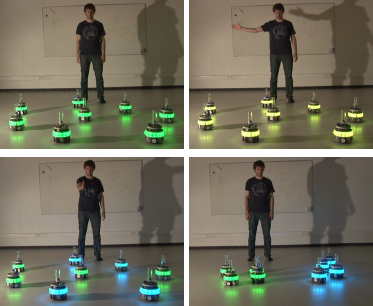
\includegraphics[scale=1]{SelfOrganisedFeedback.png}
 \decoRule
 \caption[Self Organised Feedback. \cite{Podevijn:2012}]{Self-organised, colour-based feedback during a selection and grouping task. \cite{Podevijn:2012}}
 \label{fig:SelfOrganisedFeedback}
 \end{center}
\end{figure}

McLurkin et al. \cite{McLurkin:2006} discuss the practical considerations of interfacing a human operator with their large swarm of 112 robots. The relevant portion of this work discusses the use of ``\textit{utility software for centralised development and debugging}'' \cite{McLurkin:2006}. The authors note the success of graphical interfaces based on those found in \textit{Real Time Strategy} video games for centralised data collection and display. Their \textit{SwarmCraft} graphical user interface (GUI), shown in figure \ref{fig:SwarmCraft}, can display information received regarding individuals, groups, or the whole swarm in a number of graphical forms. The authors note that one potential issue is keeping the code for displaying the data and the code on the robot side in sync, such that the GUI can always correctly display the received data. The idea of a standardised data transfer format investigated by this project could provide a potential solution to this issue. The authors go on to discuss the problem of using monitors to display the robots' internal state information when debugging group behaviours, as a user must continuously switch between watching the swarm and looking at the monitor for detailed information. The authors use a `global output' system of LEDs and sounds to solve this issue. This output is however inherently limited by the amount of information that can be represented using the small number of LEDs, and the quality of information acquired from a swarm of robots all generating sound at once. This approach also requires specific hardware to be present on each of the robots, such as the LEDs and a speaker. Augmented reality (AR) techniques therefore offer a potentially more powerful solution; by superimposing the information that would traditionally be found by looking at the monitor onto a view of the robots themselves, the user can access all available information without looking away from the swarm's activity. Furthermore the requirement for the global output hardware is removed, and the user does not need to learn how to correctly interpret these somewhat cryptic output systems, as an AR solution could display information in any form necessary, including text.

\begin{figure}
 \begin{center}
 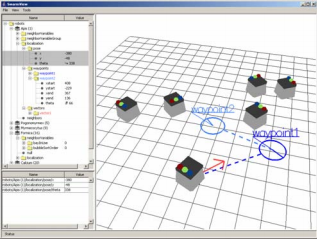
\includegraphics[scale=1]{SwarmCraft.png}
 \decoRule
 \caption[Swarm Craft GUI. \cite{McLurkin:2006}]{A screenshot of the \textit{SwarmCraft} GUI, developed by McLurkin et al. \cite{McLurkin:2006}}
 \label{fig:SwarmCraft}
 \end{center}
\end{figure}

%----------------------------------------------------------------------------------------

\section{Robotics Debugging} \label{RoboticsDebugging}
`\textit{Debugging}' is the name given to the process of fixing problems or issues (commonly referred to as bugs) in a piece of software. Well established tool-sets and techniques exist for debugging traditional software, however debugging robotic systems is a fundamentally different and more complex problem, as discussed in section \ref{ProjectContext}. The literature reviewed in this section examines the challenges of robotics debugging, and presents some tools and techniques for reducing the difficulty of this task.

Collet and MacDonald \cite{Collet:2006} describe in detail the difficulties in debugging robotics systems. The authors identify that the difficulties in developing and debugging robotics applications when compared to traditional software arise from either the environment of the robot - which will often be ``\textit{uncontrolled}'' and ``\textit{dynamic}'' - or from the mobile nature of the robot. Because the environment a given robot operates in is a real world space, the level of control that can be exerted over it by the researcher or operator is inherently limited \cite{Collet:2006}. The environment may therefore change over time, exhibit imperfections, and include other time-varying elements. A robot is a physical actor and will likely experience dynamic change in its sensor readings and its relationship to the environment over time. This is especially true for mobile robots, whose position and orientation will change over time. The behaviour of the robot often largely depends on these highly variable factors, and therefore replicating a given behaviour exactly becomes almost impossible. The authors go on to state that difficulties in debugging often arise from ``\textit{the programmer's lack of understanding of the robot's world view} \cite{Collet:2006}''. It can therefore be extrapolated that for a multi robot system such as a robot swarm this problem would be exacerbated. Each robot will have its own perception of the environment, which will differ based on differences in the robots' positions and orientations as well as variations in the instrumentation of each robot. For a multi-robot system the programmer is required to have an understanding of not just one but multiple world views, adding yet more potential for error and inaccuracy, and further obscuring bugs or behavioural issues that the programmer is trying to diagnose. This work \cite{Collet:2006} suggests that developers will need specific tools which enhance their understanding of the robots' world view in order to develop effectively for swarm robotic platforms. This need forms the mandate for the majority of this project. Collet and MacDonald \cite{Collet:2006} go on to discuss the use of augmented reality to satisfy this need, and present an augmented reality based software tool for this purpose, which is discussed in Section \ref{AugmentedReality}.

Gumbley and MacDonald \cite{Gumbley:2009} identify one of the core issues in debugging robotic behaviours using traditional debugging software to be the assumption of a ``\textit{deterministic, suspendable environment}''. This assumption rarely holds true for robots, due to their existence in a real world environment. The authors note that traditional debugging constructs such as breakpoints pause code execution, but cannot for obvious reasons also pause a robot's environment. This allows the robot's environment to change whilst execution is paused, therefore affecting the robot's behaviour. In the case where a breakpoint has been inserted to try to isolate the cause of a previously observed fault, this change in behaviour may also stop the fault from occurring. The authors \cite{Gumbley:2009} go on to consider a number of possible methods by which a developer can obtain information without pausing execution, including live data extraction which is the method chosen in this project. They note that adding code to extract information without pausing execution has the potential to affect robot behaviour. This is a salient point, and should be considered when implementing the robot-side portion of this project, where care must be taken to minimise the affect data reporting has on the execution of the robot's actual behaviour. Issues of this nature could be caused by the data reporting code taking too long to execute, thus disrupting robot behaviour. Keeping the data reporting code lightweight and efficient should therefore be a priority.

\begin{figure}
 \begin{center}
 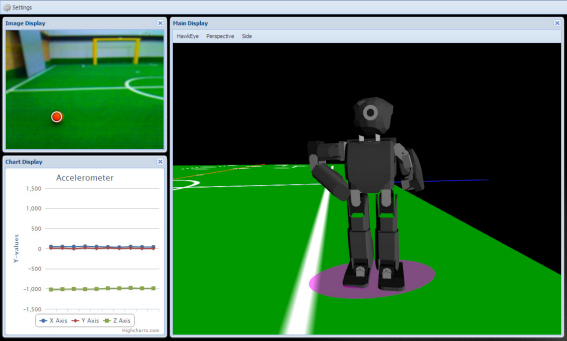
\includegraphics[scale=0.8]{NUbugger.png}
 \decoRule
 \caption[\textit{NUbugger} GUI. \cite{Annable:2014}]{The \textit{NUbugger} GUI, a real time, visual, robotics debugging utility developed by Annable et al. \cite{Annable:2014}}
 \label{fig:NUbugger}
 \end{center}
\end{figure}

In their `\textit{NUbugger}' system \cite{Annable:2014}, Annable, Budden and Mendes implement a real time, visual debugging system for robotics. The authors begin by noting that the continually increasing complexity of robotic hardware and software has lead to typical debugging approaches based on diagnosis via observation of high-level symptoms becoming increasingly less useful. They note the need for real time, visual tools, to reflect the active, physical nature of robots. The authors system \cite{Annable:2014} streams all critical system information from their robot to a web server in real time, where it can be viewed in a graphical client. The graphical interface, shown in figure \ref{fig:NUbugger}, includes a visualisation of the humanoid robot position, orientation and pose, based on its own self-localisation belief and servomotor sensor readings. It also includes a live feed from the robot's built in camera, and graphs of real time sensor data. The system has been used to diagnose a number of real, low-level issues \cite{Annable:2014} relating to the robot's image processing and object detection functionalities, demonstrating the effectiveness of real time, visual debugging tools. The use of a web server in the authors' implementation \cite{Annable:2014} allows for the collection of information regarding multiple robots, and the display of this information in multiple clients, making the system highly versatile. However one possible limitation introduced as a result is the need for a number of relatively complex networking libraries to be running on the robots, and a high connection bandwidth, in order to send the required information, limiting the system to use on relatively complex, high performance robot platforms. The system is also only targeted at a single robot platform.

%----------------------------------------------------------------------------------------

\section{Augmented Reality and Single-Robot Systems} \label{AugmentedReality}
Augmented Reality (AR) is the term used to describe the process of super-imposing `virtual' objects and elements, in the form of computer generated graphics, on to a live video image of the real world \cite{Azuma:1997}. The general aim of any augmented reality system is to give the impression that the virtual objects being rendered are actually situated within the user's real environment, and to allow the user to interact with them as such. True AR is sometimes defined as requiring the use of a \textit{head-mounted display} (HMD), as this leads to much more immersive qualities akin to virtual reality, to which AR is closely related. However this is not a universal requirement, and in one of the most widely cited surveys of the topic, Azuma \cite{Azuma:1997} provides a definition which states only three requirements of an AR system; the combination of virtual and real content, real time interaction, and 3D rendering. Figure \ref{fig:ARBasic} shows the example image used in Azuma's \cite{Azuma:1997} survey. It includes a view of a real table, augmented by virtual furniture.

\begin{figure}[h]
	\begin{center}
	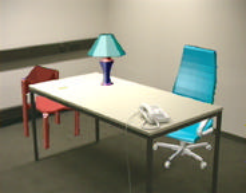
\includegraphics[scale=1.2]{ARBasic.png}
	\decoRule
	\caption[Simple AR visualisation. \cite{Azuma:1997}]{A simple example of an AR lamp and chairs augmenting a real table. \cite{Azuma:1997}}
	\label{fig:ARBasic}
	\end{center}
\end{figure}

Augmented reality presents a powerful tool for debugging robots as it allows information gathered by a robot about an environment to be superimposed onto a real world view of that environment, such that discrepancies and inconsistencies between this information and the real world become inherently obvious. More generally, augmented reality can be used to create a shared space between a human and a robot. Even as early as 1997, Azuma \cite{Azuma:1997} notes that augmented reality has a potential application in robot path planning. One limitation of Azuma's survey is its age, as the two decades since its publication have seen rapid development in computing power and computer graphics, as well as augmented reality hardware. High fidelity, consumer HMDs, such as the \textit{Microsoft HoloLens} shown in figure \ref{fig:HoloLens}, have been beginning to emerge into use within real world applications since the mid-to-late 2010s \cite{HoloLens}. A more recent survey of the topic from 2014 \cite{Billinghurst:2014} agrees with many of Azuma's earlier definitions, but provides many examples of new applications of AR technologies. The author notes the power of AR as a new paradigm for human computer interaction, and the wealth of potential application areas, including robotics.

\begin{figure}
	\begin{center}
	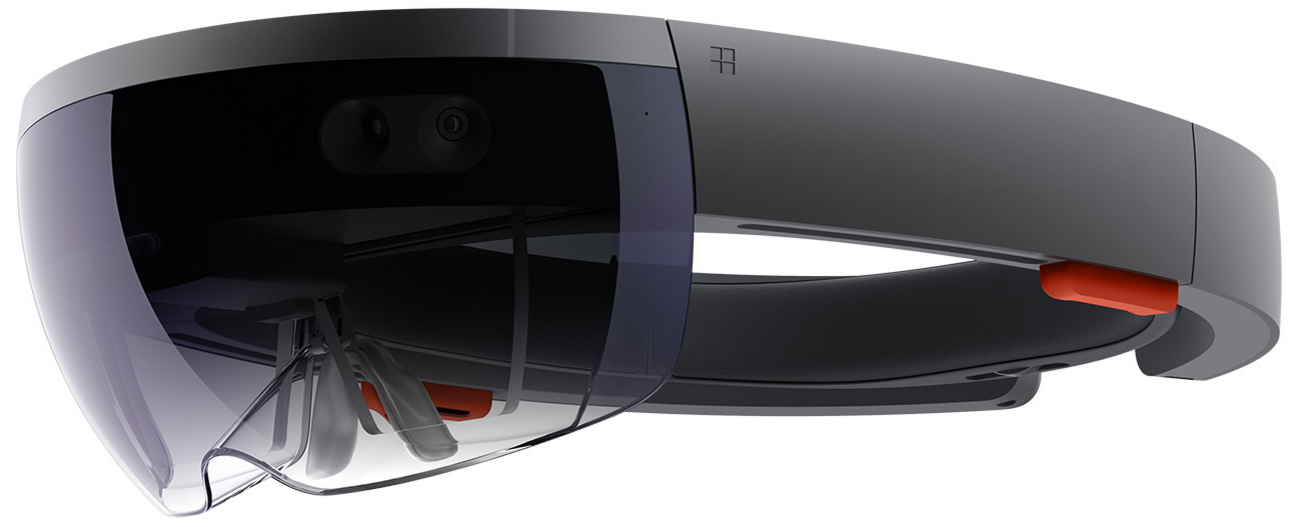
\includegraphics[scale=0.4]{HoloLens.png}
	\decoRule
	\caption[Microsoft HoloLens. ]{The Microsoft HoloLens head mounted display.}
	\label{fig:HoloLens}
	\end{center}
\end{figure}

Milgram et al. \cite{Milgram:1993} discuss the different communication formats used to interface between humans and robots, grouping them into ``\textit{continuous}'' and ``\textit{discrete}'' formats. For any communication involving a spatial or temporal component, the process of converting to and from a discrete format in order to transmit this information is an unnecessary burden. Both humans and robots use the continuous spatial dimensions, and humans have an inherent, instinctive understanding of physical things expressed in three dimensions. The authors \cite{Milgram:1993} therefore identify that  augmented reality provides an excellent means of supporting the communication of spatial information. Their paper focuses on the combination of stereoscopic displays and computer generated graphics to allow for more intuitive control of robotic systems. In the case of this project the concept is reversed; robots reporting spatial information for validation by a user should do so in a format which is inherently continuous such as a graphical visualisation in AR, rather than one that is discrete such as text-based numerical output. This should in theory reduce the time required for a human to process the information. The authors note \cite{Milgram:1993} that the ideal system utilises both discrete and continuous formats where appropriate to best communicate the required information, and is ergonomically designed to allow the user to make use of both easily and intuitively.

Like much of the HSI literature surveyed, this paper \cite{Milgram:1993} is focused primarily on robot control, rather than observation and monitoring. In spite of this much of the content of the paper remains applicable. Since the paper was written, just over twenty five years ago, major advancements have been made in virtually every area mentioned, including the quality and precision of robotic systems, their cognitive, perceptive and decision making abilities, augmented reality technologies and robotic autonomy. Because of this, some of the content of the paper has fallen out of date. Specifically, the assumption that robots lack the level of autonomy required to survey their environment and then form and execute a series of steps to carry out a relatively high level task, such as ``find and go to object Q''\cite{Milgram:1993}, is no longer necessarily true. A number of modern robots possess sufficient sensing capabilities, processing power and cognitive programming to perform such tasks based on high level commands. This does not however devalue the AR methods discussed within, and given the increased complexity and sensing capabilities of modern robots, AR based methods of interaction actually have more potential than ever. The paper however makes no mention of the potential for an AR system to report data from a robot's sensors visually, which may be attributed to the technological limitations of the time rather than an oversight by the authors.

Collet and MacDonald \cite{Collet:2006} suggest that augmented reality tools can address and mitigate some of the robotics debugging issues discussed in section \ref{RoboticsDebugging} by superimposing graphical representations of the robot's understanding of the environment on top of a live view of the environment itself \cite{Collet:2006}. Hence the programmer is able to see how the robot has interpreted the environment, and identify inconsistencies. The authors describe the image of the real world environment as the ``\textit{ground truth}'' against which the robot's view can be compared and contrasted \cite{Collet:2006}. Figure \ref{fig:Sonar} shows a visual example of this technique, where the data received from the robot's sonar sensors is converted to spatially situated 3D shapes and superimposed over the live image, and can therefore be verified visually by the user.

\begin{figure}
	\begin{center}
	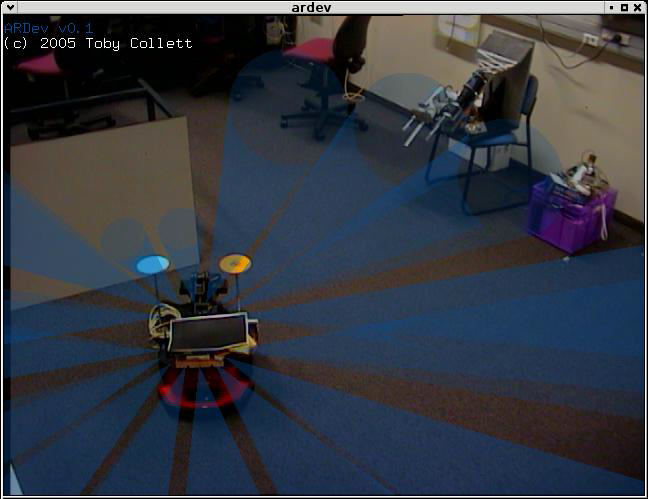
\includegraphics[scale=0.6]{Sonar.png}
	\decoRule
	\caption[Sonar data visualisation. Collet and MacDonald \cite{Collet:2006}]{Sonar sensor data visualisation in Collet and MacDonald's system \cite{Collet:2006}.}
	\label{fig:Sonar}
	\end{center}
\end{figure}

The application developed during this project closely follows this paradigm; allowing the user to identify bugs by comparing the robot's knowledge of its environment and its decision making factors (collectively referred to as its state) with a view of the environment, in real time. The application aims to apply this concept specifically to swarm robotics systems, and therefore must allow the user to compare the states of multiple robots with the environment simultaneously. From the perspective of each robot in the swarm, the other robots will form part of the environment, therefore the application must take this into account when displaying the information. Because of the large increase in information from a single-robot system to a multi-robot one, it becomes important that the application provides a way for the user to filter what information is displayed, allowing them to focus on the primary aspect under test. Filtering also allows the user to compare and contrast specific robots against one another by filtering out information related to other robots, or by displaying in more detail information related to the robots of interest.

\section{Augmented Reality and Multiple-Robot Systems} \label{SimilarWork}
A number of pieces of research have investigated different ways to monitor and interact with multi-robot systems, using a combination of augmented reality technology and HSI techniques. These similar works are summarised and reviewed in this section.

Daily et al. \cite{Daily:2003} present a technique for retrieving information from a swarm of robots, and displaying this to a user in a ``\textit{world-embedded}'' manner using augmented reality techniques. One of the stated aims of this work was the use of minimal communication bandwidth. The authors present \cite{Daily:2003} an infra-red (IR) LED based solution for both indicating robot position, and communicating a small amount of information, in the form of coded pulse sequences, simultaneously. The HMD worn by the user decodes this information and superimposes a graphical representation on top of the user's view of the robots using a see-through optical display. Communicating via IR LED directly to the user's HMD removes the need for communication infrastructure, however it requires the user to have a direct line-of-sight to the robots in order to receive information. The data rate that can be achieved via this method is also heavily limited. However in the use case demonstrated by the authors \cite{Daily:2003}, involving the display of a gradient in the direction of a target known to the swarm, the system is effective. The hardware requirements for this system are quite specific, and unlikely to be available on most robotics platforms, however the power of this kind of spatially situated or world-embedded data visualisation is clear.

Ghiringhelli et al. \cite{Ghiringhelli:2014} present a system for augmenting a video feed of an environment containing a number of robots with real time information obtained from each of the robots. This is similar in concept to the system described by Collet and MacDonald \cite{Collet:2006}, but is designed specifically to target a multi-robot system. The authors identify the ability to overlay spatial information exposed by the robots on to the video feed in real time, in the form of situated graphical representations, as the most important debugging feature of the system. Figure \ref{fig:SpatiallySituated} shows a spatially situated overlay of data exposed by robot thirty two, in the authors' system \cite{Ghiringhelli:2014}. A viewer is able to immediately verify the validity of the robot's world view from this image by comparing the blue overlay to the image beneath. Each robot features a coloured LED blinking a unique coded pattern to enable tracking, and the system uses homography techniques to map between each robot's frame of reference and the camera's \cite{Ghiringhelli:2014}. The author's system therefore requires hardware to be present on the robots to support the tracking method. The homography technique also requires a reference frame to be established on the floor of the robot space. The system developed in this project uses a simpler approach, with position and orientation tracking achieved through the use of the ArUco \cite{Garrido:2014} marker-based tracking system. The camera is positioned with a bird's-eye view of the space, to simplify mapping by effectively reducing the 3D space to a 2D approximation. The tracking LEDs used by the authors' system \cite{Ghiringhelli:2014} are active components, and therefore require specific hardware to be available on the robots in order for them to be tracked. This limits the system's generalisability. In contrast, using a passive, marker based technique means that no specific hardware is required, and the tracking could in theory be performed on any robot to which a marker can be attached.

\begin{figure}
	\begin{center}
	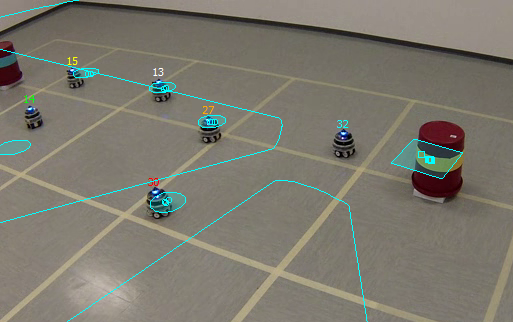
\includegraphics[scale=0.8]{SpatiallySituatedData.png}
	\decoRule
	\caption[Spatially situation data overlay. Garrido et al. \cite{Ghiringhelli:2014}]{Example of spatially situated data overlayed on a live image in \cite{Ghiringhelli:2014}.}
	\label{fig:SpatiallySituated}
	\end{center}
\end{figure}

The authors \cite{Ghiringhelli:2014} also note the inclusion of a number of interaction modalities which allow the user to manipulate the visibility and display of specific elements of the data, which is grouped according to its associated robot and its type. This allows a user to focus only on pertinent information by hiding other information which is irrelevant. This follows the guidelines established in Rule and Forlizzi's work \cite{Rule:2012} on HSI, and the requirements of users regarding information salience and display when interacting with multi robot systems. Following this precedent, display configuration was identified as a priority and implemented within the system described in this project. This project also looks at expanding the methods used to display data to include more standard interface elements not directly related to the video image, as previously seen in \cite{McLurkin:2006}, which is not addressed in \cite{Ghiringhelli:2014}. Overall Ghiringhelli et al. \cite{Ghiringhelli:2014} demonstrate how effective augmented reality-based tools can be for debugging a multi-robot system, and this project attempts to build on this success by providing a more generalised tool, which can meet the requirements of a large number of swarm-robotics systems.

\section{Summary}
The system developed during this project seeks to combine a number of ideas and techniques from existing systems and previous work to create a tool which specifically benefits swarm robotics development, but is generalisable in terms of target platform and required hardware. The system aims to collect and display swarm data in a central GUI similar to \cite{McLurkin:2006}, in the spatially situated, AR-based manner of \cite{Collet:2006}, \cite{Daily:2003}, and \cite{Ghiringhelli:2014}. The system is generalised by avoiding the specific hardware requirements of \cite{McLurkin:2006} and \cite{Collet:2006}, which tie those systems to specific platforms, and by using communication technologies which are more standard and more commonly understood than in \cite{Daily:2003}, and more flexible and information rich than in \cite{Podevijn:2012}. The use of a standardised, defined data format helps avoid some of the code synchronization issues of \cite{McLurkin:2006}, and aids in keeping the system general. Specific concepts regarding the display of data, as described in \cite{Rule:2012} and applied in \cite{Ghiringhelli:2014} are also considered and applied within this system. Overall this project aims to help further efforts to improve human-swarm interaction, and add to the available set of swarm debugging tools one that is easy to understand, simple to extend, and well generalised such that it might be ported to different robot platforms in future. It is hoped that the software developed will be useful within the work of the YRL, as well as having scope for extension and use by the wider swarm robotics community.
